%\documentclass[11pt,a4paper]{article}
%\usepackage{fullpage}
%\usepackage{beamerarticle}
%\documentclass[handout,xcolor=pdftex,dvipsnames,table]{beamer}
\documentclass[hyperref={unicode=true}]{beamer}

%\usepackage{pgfpages} 
%\pgfpagesuselayout{resize}[a4paper,border shrink=5mm,landscape] 

\usepackage[utf8]{inputenc}
\usepackage[russian]{babel}
\usepackage{../clrscode3e} 
%\usepackage[all]{xy}
\usepackage{colortbl}
%\usepackage{xcolor}
\usepackage{pstricks, pst-tree, pst-node}
\usepackage{epsfig}
\usepackage{multicol}
\usepackage{array}
\usepackage{wrapfig}
%\usepackage{listings}

\definecolor{orange}{cmyk}{0,0.52,1,0}

%\usepackage{beamerthemesplit}

\AtBeginSection[]
{
  \begin{frame}<beamer>{Раздел}
    \tableofcontents[currentsection]
  \end{frame}
}


\AtBeginSubsection[]
{
  \begin{frame}<beamer>{Раздел}
    \tableofcontents[currentsection,currentsubsection]
  \end{frame}
}


\newtheorem{rtheorem}{Теорема} 
\newtheorem{rconsequence}{Следствие} 
\newtheorem{rdefinition}{Определение} 
%default}
%themesplit}

\title{Жадные алгоритмы}
\subtitle{Дискретный анализ 2012/13}
\author{Андрей Калинин, Татьяна Романова}
\date{16 марта 2013 г.}
\usetheme{default}
%\usefonttheme{serif}
\usefonttheme[onlymath]{serif}
%\usefonttheme{professionalfonts}
%\usetheme{default} 


\begin{document}

\frame{\titlepage}

\frame
{
  \frametitle{Литература}


  \begin{itemize}
  \item  Кормен Т., Лейзерсон Ч., Ривест Р., Штайн К.. Алгоритмы:
    построение и анализ, 2-е издание, М.:Вильямс, 2005, стр. 442-478, 
    глава 16, <<Жадные алгоритмы>>. 
  \item Дэн Гасфилд, <<Строки деревья и последовательности в алгоритмах:
    Информатика и вычислительная биология>>, 2003. Глава 12,
    <<Улучшение процедур выстраивания>>, стр. 351--359.
  \end{itemize}
}

%\section[Содержание]{}
\frame{\tableofcontents}

\section{Жадные алгоритмы}

\frame{
  \frametitle{Идея}
  \begin{itemize}
  \item Похожи на динамическое программирование, используются для
    решения задач оптимизации. 
  \item Когда приходит необходимость сделать выбор, то делается выбор
    такого решения, которое кажется лучшим {\em сейчас}. Надеемся, что
    локально-оптимальный выбор приведёт к глобально-оптимальному
    решению. 
  \item Жадные алгоритмы далеко не всегда дают оптимальное
    решение. Однако, в тех случаях, когда они всё-таки приводят к
    нему, они работают за очень короткое время. 
  \item Рассмотрим задачи, решаемые <<жадным>> способом и определим область
    применимости жадных алгоритмов. 
  \end{itemize}
}

\subsection{Задача о выборе процессов}

\frame{
  \frametitle{Постановка задачи}
  \begin{itemize}
  \item Есть $n$ процессов, требующих эксклюзивного использования
    общего ресурса (например лекции в аудитории).
  \item $S = \{a_1, \ldots, a_n \}$.
  \item $a_i$ требует ресурс на период $[s_i, f_i)$.
  \item Нужно выбрать наибольшее возможное множество неперекрывающихся
    по использованию ресурса
    процессов. 
  \item В задачах о расписаниях могут быть другие цели: занять
    компнату на самое длительное время, максимизировать доход от аренды и
    т.п. 
  \end{itemize}
}

\frame{
  \frametitle{Пример}
  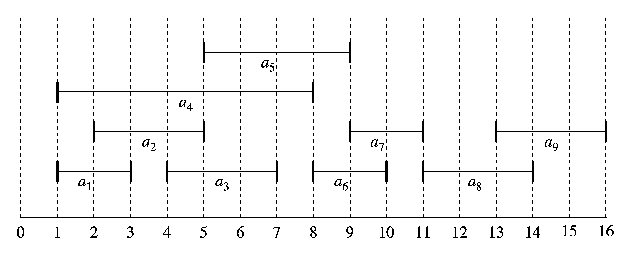
\includegraphics{act-sel-1.eps}\\
~\\
~\\
\begin{columns}
\begin{column}{.6\textwidth}
  \begin{tabular}{r|ccccccccc|}
    $i$ & 1 & 2 & 3 & 4 & 5 & 6 & 7 & 8 & 9 \\
    \hline
    $s_i$ & 1 & 2 & 4 & 1 & 5 & 8 & 9 & 11 & 13 \\
    $f_i$ & 3 & 5 & 7 & 8 & 9 & 10 & 11 & 14 & 16
  \end{tabular}
\end{column}
\begin{column}{.4\textwidth}
  Множества: $\{a_1, a_3, a_6, a_8\}$; $\{ a_2,
  a_5, a_7, a_9\}$.
\end{column}
\end{columns}
}

\frame{
  \frametitle{Оптимальная подструктура}
  \begin{itemize}
    \item Количество процессов, начинающихся после окончания $a_i$ и
      заканчивающихся перед началом $a_j$:
 \[
 S_{ij} = \{ a_k\in S~ |~f_i \leq s_k < f_k \leq s_j\}
\]
\item Процессы в $S_{ij}$ совместны со всеми другими процессами, которые
  заканчиваются до $f_i$ и начинаются после $s_j$.
\item  Добавим фиктивные процессы:
  \[
  \begin{split}
    a_0 =& [-\infty, 0) \\
    a_{n+1} =& [\infty, \infty +1)
  \end{split}
\]
\item $S = S_{0,n+1}$.
\end{itemize}
}

\frame{
  \frametitle{Оптимальная подструктура}
  \begin{itemize}
    \item Предположим, что все процессы отсортированы по возрастанию
      времени окончания:
      \[
      f_0 \leq f_1 \leq f_2 \cdots \leq f_n \leq f_{n+1}.
      \]
    \item Тогда для $i \geq j$ $S_{ij} = \emptyset$. Предположим
      обратное:
      \begin{enumerate}
        \item Если существует $a_k \in S_{ij}$, то 
          \[
          f_i \leq s_k < f_k \leq s_j < f_j \quad \Rightarrow \quad
          f_i < f_j
          \]
          \item Но из $i \geq j$ должно следовать $f_i \geq f_j$,
            т.е. противоречие.
      \end{enumerate}
      То есть, нужно рассматривать только $S_{ij}$ для котрых $0 \leq
      i < j \leq n+1$
  \end{itemize}
}

\frame{
  \frametitle{Оптимальная подструктура}
  Допустим, оптимальное решение $A_{ij}$ для $S_{ij}$ включает в себя $a_k$. Тогда есть две
  подзадачи: 
  \begin{itemize}
    \item Найти оптимальное решение $A_{ik}$ для $S_{ik}$. 
    \item Найти оптимальное решение $A_{kj}$ для $S_{kj}$.
  \end{itemize}
  Необходимость оптимального решения доказывается от противного. Тем
  самым:
  \[
  A_{ij} = A_{ik} \cup \{a_k\} \cup A_{kj}
  \]
}

\frame{
  \frametitle{Рекурсивное решение}
  \begin{itemize}
    \item $c[i,j] = |A_{ij}|$.
    \item Если $a_k\in A_{ij}$, то
\[
c[i,j] = c[i,k] + c[k,j] + 1.
\] 
\item Тем самым:
\[
c[i,j] = \left\{ 
  \begin{array}{ll}
    0 & S_{ij} = \emptyset \\
    \displaystyle\max_{i < k < j \atop a_k \in S_{ij}} \{ c[i,k]+c[k,j] +
    1\} & S_{ij} \neq \emptyset
  \end{array}
\right.
\]
  \end{itemize}
\pause
Далее просто решить задачу методом динамического программирования, но
мы пойдём иным путём. 
}

\frame{
  \frametitle{Обоснование жадного выбора}

  \begin{rtheorem}
    Расмотрим произвольную непустую задачу $S_{ij}$ и пусть $a_m$ ---
    процесс, который заканчивается раньше других:
\[
f_m = \min\{ f_k~|~a_k \in S_{ij}\}.
\]
В этом случае справедливы такие утверждения:
\begin{enumerate}
\item Процесс $a_m$ используется в некоторм подмножестве максимального
  размера, состоящем из взаимно совместимых процессов задачи $S_{ij}$.
\item Подзадача  $S_{im}$ пустая, поэтому в результате выбора процесса
  $a_m$ непустой остаётся только подзадача $S_{mj}$.
\end{enumerate}
  \end{rtheorem}
}

\frame{
  \begin{proof}
    \begin{itemize}
      \item[2.] Допустим, $a_k \in S_{im}$. Тогда $f_i \leq s_k < f_k
        \leq s_m < f_m \Rightarrow f_k <f_m$. Т.е., $a_k \in S_{ij}$ и
        заканчивается раньше $f_m$, что противоречит выбору
        $a_m$. Следовательно не существует $a_k \in S_{im} \Rightarrow
        S_{im} = \emptyset$.
      \item[1.] Покажем, что $a_m$ входит в одно из решений задачи
        $S_{ij}$:
        \begin{itemize}
        \item Организуем процессы в $A_{ij}$ в порядке возрастания
          времени окончания. 
        \item $a_k$ --- первый процесс в $A_{ij}$.
        \item Если $a_k = a_m$, то то утверждение доказано. 
        \item Иначе, сделаем $A'_{ij} = A_{ij} - \{a_k\} \cup \{a_m\}$
          (заменим $a_k$ на~$a_m$).
        \item Процессы в $A'_{ij}$ не перекрывается, т.к. $f_m \leq
          f_k$.
        \item $|A_{ij}| = |A'_{ij}|$, т.е. $A'_{ij}$ --- подмножество
          максимального размера, включающее в себя процесс $a_m$.
        \end{itemize}
    \end{itemize}
  \end{proof}
}

\frame{
  \frametitle{Жадный выбор}
  Чтобы решить задачу $S_{ij}$:
  \begin{itemize}
  \item  Найдём $a_m \in S_{ij}$ с наименьшим временем окончания --- 
    жадный выбор. 
  \item Решим задачу $S_{mj}$.
    Последовательно выбираем процессы, проходя по ним в порядке
    возрастания времени окончания. 
  \end{itemize}
}

\frame{
  \frametitle{Рекурсивный алгоритм}
  \begin{codebox}
    \Procname{$\proc{Rec-Activity-Selector}(s,f,i,n)$}
    \li $m \gets i+1$
    \li \While $m \leq n$ \id{and} $s_m < f_i$ \Do
    \li $m \gets m+1$ \End
    \li \If $m \leq n$
    \li \Then \Return $\{ a_m \} \cup
    \proc{Rec-Activity-Selector}(s,f,m,n)$
    \li \Else \Return $\emptyset$ \End
  \end{codebox}
}

\frame{
  \frametitle{Итеративный алгоритм}
  \begin{codebox}
    \Procname{$\proc{Greedy-Activity-Selector}(s,f,i,n)$}
    \li $A \gets \{ a_1 \}$
    \li $i \gets 1$
    \li \For $m \gets 2$ \To $n$ \Do
    \li \If $s_m \geq f_i$
    \li \Then $A \gets A \cup \{ a_m \}$
    \li $i \gets m$ \End \End
    \li \Return $A$
  \end{codebox}
}

\subsection{Элементы жадной стратегии}

\frame{
  \frametitle{Что было сделано?}
  \begin{enumerate}
  \item Определена оптимальная подструктура задачи. 
  \item Разработано рекурсивное решение. 
  \item Доказано, что на любом этапе рекурсии один из оптимальных
    выбров является жадным.
  \item Показано, что все возникающие в результате жадного выбора
    подзадачи, кроме одной, --- пустые. 
  \item Разработан рекурсивный алгоритм, реализующий жадную
    стратегию. 
  \item Рекурсивный алгоритм преобразован в итеративный. 
  \end{enumerate}
}

\frame{
  \frametitle{Процесс разработки жадных алгоритмов}
  \begin{enumerate}
  \item Привести задачу оптимизации к виду, когда после сделанного
    выбора остаётся решить только одну подзадачу. 
  \item  Доказать, что всегда существует такое оптимиальное решение
    исходной задачи, которое можно получить путём жадного выбора, так
    что такой выбор всегда допустим. 
  \item Показать, что после жадного выбор остаётся подзадача,
    обладающая тем свойством, что объединение оптимального решения
    подзадачи со сделанным жадным выброром приводит к оптимальному
    решению исходной задачи. 
  \end{enumerate}
}

\frame{
  \frametitle{Свойство жадного выбора}
  Глобальное оптимальное решение можно получить, делая локальный
  оптимальный (жадный) выбор. Для динамического программмирования: 
  \begin{itemize}
    \item На каждом шаге делается выбор. 
    \item Выбор зависит от известных оптимальных решений для подзадач,
      т.е. сначала нужно решить подзадачи. 
    \item Порядок решения <<снизу-вверх>>.
  \end{itemize}
  Для жадного выбора:
  \begin{itemize}
  \item На каждом шаге делается выбор. 
  \item Выбор делается перед решением подзадач. 
  \item Порядок решения <<сверху-вниз>>.
  \end{itemize}
}

\frame{
  \frametitle{Оптимальная подструктура}

  Для применимости жадных алгоритм требуется, как и в динамическом
  программировании, наличие оптимальной подструктуры в задаче. 
}

\frame{
  \frametitle{Сравнение жадных алгоритмов и динамического
    программирования}
  \begin{itemize}
  \item Дискретная задача о рюкзаке: Вор во время ограбления магазина
    обнаружил $n$ предметов. Предмет под номером $i$ имеет стоимость
    $v_i$ и вес $w_i$, где $v_i$ и $w_i$ --- целые числа. Нужно унести
    вещи, суммарная стоимость которых была бы как можно большей,
    однако грузоподъёмность рюкзака ограничивается $W$
    килограммами. Какие предметы следует взять с собой?
  \item Непрерывная задача о рюкзаке та же, но теперь тот или иной
    товар вор может брать с собой частично, а не делать каждый раз
    бинарный выбор.  
  \end{itemize}
}

\frame{
  \frametitle{Задачи о рюзкаке: оптимальная подструктура}

  В дискретной задаче есть оптимальная подструктура: 
  \begin{itemize}
  \item Допустим, есть оптимальное решение задачи для рюкзака весом
    $W$.
  \item Если из рюкзака вынуть $j$-ый предмет, то остальные предметы
    должны быть наиболее ценными, вес которых не превышает $W-w_j$ и
    которые можно составить из $n-1$ исходных предметов. 
  \end{itemize}
  Для непрерывной задачи рассуждения аналогичны. 
}

\frame{
  \frametitle{Жадное решение задач о рюкзаке}
  \begin{itemize}
  \item Отсортируем вещи по <<удельной ценности>>, $v_i/w_i$.
  \item Будем последовательно выбирать вещи с максимальной удельной
    ценностью и помещать их в рюкзак. 
  \end{itemize}
\pause
  Такое решение работает для непрерывной задачи о рюкзаке и не
  работает для дискретной. Например, $W=50$:\\
~\\
~\\
\begin{columns}
\begin{column}{.5\textwidth}
  \begin{tabular}{r|ccc}
    $i$ & 1 & 2 & 3 \\
    \hline 
    $v_i$ & 60 & 100 & 120 \\
    $w_i$ & 10 & 20 & 30 \\
    $v_i/w_i$ & 6 & 5 & 4
  \end{tabular}
\end{column}
\begin{column}{.5\textwidth}
Жадное решение: вещи 1 и 2, сумма 160, вес 30. 
Оптимальное решение: вещи 2 и 3, сумма 220, вес 50. 
\end{column}
\end{columns}
}

\subsection{Коды Хаффмана}

\begin{frame}
\frametitle{Пример}
Допустим, есть файл, состоящий из 100\,000 символов, который нужно
сжать:\\
~\\
\begin{tabular}{l|cccccc}
 & a & b & c & d & e & f \\
\hline
Частота (в тысячах) & 45 & 13 & 12 & 16 & 9 & 5 \\
Фикс. длина & 000 & 001 & 010 & 011 & 100 & 101 \\
Перемен. длина & 0 & 101& 100 & 111 & 1101 & 1100
\end{tabular} \\
~\\
~\\
При использовании кода фиксированной длины понадобится 300\,000 битов;
с помощью кода переменной длины потребуется
\[
(45\cdot 1 + 13\cdot 3 + 12\cdot 3 + 16\cdot 3 + 9\cdot 4 + 5\cdot
4)\cdot 1000 = 224\,000
\]
\end{frame}

\begin{frame}
\frametitle{Префиксные коды}
\begin{itemize}
\item Префиксный код --- код, в котром ни одно кодовое слово не является
префиксом другого кодового слова. 
\item Тогда кодирование текста --- конкатенация всех кодов символов. 
\item Префиксные коды упрощают декодирование. 
\item Код можно представить в виде дерева. 
\end{itemize}
\end{frame}

\begin{frame}
\begin{tabular}{l|cccccc}
 & a & b & c & d & e & f \\
\hline
Частота (в тысячах) & 45 & 13 & 12 & 16 & 9 & 5 \\
Фикс. длина & 000 & 001 & 010 & 011 & 100 & 101 \\
Перемен. длина & 0 & 101& 100 & 111 & 1101 & 1100
\end{tabular} \\
~\\
\pstree[levelsep=40pt]{\Toval{100}}{
  \pstree{\Tcircle{86}^{0}}{
    \pstree{\Tcircle{58}^{0}}{
      \Tr{\psframebox{a:45}}^{0}
      \Tr{\psframebox{b:13}}_{1}
    }
    \pstree{\Tcircle{28}_{1}}{
      \Tr{\psframebox{c:12}}^{0}
      \Tr{\psframebox{d:16}}_{1}
    }
  }
  \pstree{\Tcircle{14}_{1}}{
    \pstree{\Tcircle{14}^{0}}{
      \Tr{\psframebox{e:9}}^{0}
      \Tr{\psframebox{f:5}}_{1}
    }
  }
}

\end{frame}

\begin{frame}[plain]
\begin{tabular}{l|cccccc}
 & a & b & c & d & e & f \\
\hline
Частота (в тысячах) & 45 & 13 & 12 & 16 & 9 & 5 \\
Фикс. длина & 000 & 001 & 010 & 011 & 100 & 101 \\
Перемен. длина & 0 & 101& 100 & 111 & 1101 & 1100
\end{tabular} \\
~\\
~\\
\begin{center}
\pstree[levelsep=40pt]{\Toval{100}}{
  \Tr{\psframebox{a:45}}^{0}
  \pstree{\Tcircle{55}_{1}}{
    \pstree{\Tcircle{25}^{0}}{
      \Tr{\psframebox{c:12}}^{0}
      \Tr{\psframebox{b:13}}_{1}
    }
    \pstree{\Tcircle{30}_{1}}{
      \pstree{\Tcircle{14}^{0}}{
        \Tr{\psframebox{f:5}}^{0}
        \Tr{\psframebox{e:9}}_{1}
      }
      \Tr{\psframebox{d:16}}_{1}
    }
  }
}
\end{center}

\end{frame}

\begin{frame}
\frametitle{Дерево оптимального кода}
\begin{itemize}
\item Оптимальный код текста всегда может быть представлен полным
  бинарным деревом, в котором у каждого узла (кроме листьев) имеется
  по два дочерних узла. 
\item Т.е., если $C$ --- алфавит, то дерево, представляющее
  оптимальный префиксный код, содержит ровно $|C|$ листьев и  $|C|-1$
  внутренних узлов.
\item Если есть дерево $T$ некоторого префиксного кода, то обозначив
  через $f(c)$ частоту символа $c\in C$, а через $d_T(c)$ --- глубину
  листа $c$ в дереве $T$, то для кодировки текста потребуется:
\[
B(T)=\sum_{c\in C} f(c)d_T(c).
\]
$B(T)$ --- стоимость дерева $T$.
\end{itemize}
\end{frame}

\begin{frame}
\frametitle{Построение дерева Хаффмана}
$Q$ --- очередь с приоритетами, пирамида. 
\begin{codebox}
\li $n \gets |C|$, $Q \gets C$  
\li \For $i \gets 1$ \To $n-1$ \Do
\li Выделить память для узла $z$
\li $left[z] \gets x \gets \proc{Extract-Min}(Q)$
\li $right[z] \gets y \gets \proc{Extract-Min}(Q)$
\li $f[z] \gets f[x] + f[y]$
\li $\proc{Insert}(Q,z)$ \End
\li \Return $\proc{Extract-Min}(Q)$
\end{codebox}
\end{frame}

\begin{frame}
\begin{tabular}{cccccc}
  \Tr{\psframebox{f:5}}& 
  \Tr{\psframebox{e:9}} &
  \Tr{\psframebox{c:12}} &
  \Tr{\psframebox{b:13}} &
  \Tr{\psframebox{d:16}} &
  \Tr{\psframebox{a:45}}
\end{tabular}\\
~\\
~\\
~\\
\pause
\begin{tabular}{ccccc}
  \Tr{\psframebox{c:12}} &
  \Tr{\psframebox{b:13}} &
  \pstree[levelsep=40pt]{\Tcircle{14}}{
  \Tr{\psframebox{f:5}}^{0} 
  \Tr{\psframebox{e:9}}_{1} 
  } &
  \Tr{\psframebox{d:16}} &
  \Tr{\psframebox{a:45}}
\end{tabular}\\
~\\
~\\
~\\
\pause
\begin{tabular}{cccc}
  \pstree[levelsep=40pt]{\Tcircle{14}}{
  \Tr{\psframebox{f:5}}^{0} 
  \Tr{\psframebox{e:9}}_{1} 
  } &
  \Tr{\psframebox{d:16}} &
  \pstree[levelsep=40pt]{\Tcircle{25}}{
  \Tr{\psframebox{c:12}}^{0} 
  \Tr{\psframebox{b:13}}_{1} 
  } &  
  \Tr{\psframebox{a:45}}
\end{tabular}\\
\end{frame}

\begin{frame}
\begin{tabular}{cccc}
  \pstree[levelsep=40pt]{\Tcircle{14}}{
  \Tr{\psframebox{f:5}}^{0} 
  \Tr{\psframebox{e:9}}_{1} 
  } &
  \Tr{\psframebox{d:16}} &
  \pstree[levelsep=40pt]{\Tcircle{25}}{
  \Tr{\psframebox{c:12}}^{0} 
  \Tr{\psframebox{b:13}}_{1} 
  } &  
  \Tr{\psframebox{a:45}}
\end{tabular}\\
~\\
~\\
~\\
\pause
\begin{tabular}{ccc}
  \pstree[levelsep=40pt]{\Tcircle{25}}{
  \Tr{\psframebox{c:12}}^{0} 
  \Tr{\psframebox{b:13}}_{1}
  } &
  \pstree[levelsep=40pt]{\Tcircle{30}}{
    \pstree[levelsep=40pt]{\Tcircle{14}^{0}}{
      \Tr{\psframebox{f:5}}^{0} 
      \Tr{\psframebox{e:9}}_{1} 
    } 
    \Tr{\psframebox{d:16}}_{1}
  }
  &
  \Tr{\psframebox{a:45}}
\end{tabular}
\end{frame}

\begin{frame}
\begin{tabular}{cc}
  \Tr{\psframebox{a:45}} &
  \pstree[levelsep=40pt]{\Tcircle{55}}{
  \pstree[levelsep=40pt]{\Tcircle{25}^{0}}{
  \Tr{\psframebox{c:12}}^{0} 
  \Tr{\psframebox{b:13}}_{1}
  } 
  \pstree[levelsep=40pt]{\Tcircle{30}_{1}}{
    \pstree[levelsep=40pt]{\Tcircle{14}^{0}}{
      \Tr{\psframebox{f:5}}^{0} 
      \Tr{\psframebox{e:9}}_{1} 
    } 
    \Tr{\psframebox{d:16}}_{1}
  }
}
\end{tabular}
\end{frame}

\begin{frame}
\begin{center}
  \pstree[levelsep=40pt]{\Tcircle{100}}{
  \Tr{\psframebox{a:45}}^{0}
  \pstree[levelsep=40pt]{\Tcircle{55}_{1}}{
  \pstree[levelsep=40pt]{\Tcircle{25}^{0}}{
  \Tr{\psframebox{c:12}}^{0} 
  \Tr{\psframebox{b:13}}_{1}
  } 
  \pstree[levelsep=40pt]{\Tcircle{30}_{1}}{
    \pstree[levelsep=40pt]{\Tcircle{14}^{0}}{
      \Tr{\psframebox{f:5}}^{0} 
      \Tr{\psframebox{e:9}}_{1} 
    } 
    \Tr{\psframebox{d:16}}_{1}
  }
}
}
\end{center}
\end{frame}

\frame{
  \frametitle{Обоснование жадного выбора}
  \begin{rtheorem}
    Пусть $C$ --- алфавит, каждый символ $c\in C$ которого встречается
    с частотой $f[c]$. Пусть $x$ и $y$ --- два символва алфавита $C$ с
    самыми низкими частотами. Тогда для алфавита $C$ существует
    оптимальный префиксный код, кодовые слова символов $x$ и $y$ в
    котором имеют одинаковую длину и отличаются лишь последним битом.
  \end{rtheorem}
  \begin{proof}
    \begin{itemize}
      \item $T$ --- дерево оптимального префиксного кода.
      \item $a$ и $b$ --- символы, находящиеся на максимальной глубине
        с общим родительским узлом. Предположим, что $f[a] \leq f[b]$
        и $f[x] \leq f[y]$. Тогда и $f[x] \leq f[a]$ и $f[y] \leq
        f[b]$.
    \end{itemize}
  \end{proof}
}

\frame[plain]{
\begin{tabular}{ccccccc}
$T$:
&
  \pstree[levelsep=20pt]{\Tcircle{~}}{
    \pstree{\Tcircle{~}}{
      \Tr{\psframebox{$y$}}
      \pstree{\Tcircle{~}}{
        \Tr{\psframebox{$a$}}
        \Tr{\psframebox{$b$}}
      }
    }
    \Tr{\psframebox{$x$}}
  }
&
~~~$T'$:
&
  \pstree[levelsep=20pt]{\Tcircle{~}}{
    \pstree{\Tcircle{~}}{
      \Tr{\psframebox{$y$}}
      \pstree{\Tcircle{~}}{
        \Tr{\psframebox{$x$}}
        \Tr{\psframebox{$b$}}
      }
    }
    \Tr{\psframebox{$a$}}
  }
&
~~~$T''$:
&
  \pstree[levelsep=20pt]{\Tcircle{~}}{
    \pstree{\Tcircle{~}}{
      \Tr{\psframebox{$b$}}
      \pstree{\Tcircle{~}}{
        \Tr{\psframebox{$x$}}
        \Tr{\psframebox{$y$}}
      }
    }
    \Tr{\psframebox{$a$}}
  }
\end{tabular}
  \begin{proof}
    \begin{itemize}
      \item $T'$ --- перестановка $a$ и $x$, а $T''$ -- перестановка
        $b$ и $y$. Тогда:
\[
\begin{split}
B(T) - B(T') &=  \sum_{c\in C} f(c)d_T(c) - \sum_{c\in C}
f(c)d_{T'}(c) = \\
&= f[x]d_T(x)+f[a]d_T(a)-f[x]d_{T'}(x)-f[a]d_{T'}(a) = \\
&=f[x]d_T(x)+f[a]d_T(a)-f[x]d_T(a)-f[a]d_T(x) = \\
&=(f[a]-f[x])(d_T(a)-d_T(x)) \geq 0
\end{split}
\]
\item Аналогично, $B(T')-B(T'')\geq 0$ и $B(T'')\leq B(T)$. Но должно
  так же $B(T)\leq B(T'')$, следовательно $B(T'')=B(T)$.
    \end{itemize}
  \end{proof}

}

\frame{
  \frametitle{Оптимальная подструктура}
  \begin{rtheorem}
    \begin{itemize}
      \item $x,y \in C$  --- символы  с минимальными частотами. 
      \item $C' = C - \{x,y\}\cup \{z\}$, $f[z] = f[x]+f[y]$.
      \item $T'$ --- дерево оптимального префиксного кода $C'$.
      \item Тогда дерево $T$, полученное из $T'$ путём замены листа
        $z$ внутренним узлом с сыновьями $x$ и $y$, представляет
        оптимальный префиксный код для $C$. 
    \end{itemize}
  \end{rtheorem}
}

\frame[plain]{
  \begin{proof}
    \begin{itemize}
      \item $c \in C - \{x,y\}:~d_T(c)=d_{T'}(c)$, т.е. $f[c]d_T(c) =
      f(c)d_{T'}(c)$, 
      \item $d_T(x) = d_T(y) = d_{T'}(z)+1$, тогда:
        \[
        \begin{split}
          f[x]d_T(x)+f[y]d_T(y) &= (f[x]+f[y])(d_{T'}(z)+1) = \\
          &= f[z]d_{T'}(z)+(f[x]+f[y]).
        \end{split}
        \]
      \item Следовательно, $B(T)=B(T')+f[z]+f[y]$ или
        $B(T')=B(T)-f[x]-f[y]$.
      \item  Предположим, что $T$ --- не оптимальное. Тогда существует
        оптимальное дерево $T''$, такое что $B(T'')<B(T)$. $x$ и $y$
        можно считать сыновьями одного узла и $T'''$ получено из $T''$
        заменой $x$ и $y$ листом $z$ с частотой
        $f[z]=f[x]+f[y]$. Тогда:
        \[
        B(T''')=B(T'')-f[x]-f[y]< B(T)-f[x]-f[y]=B(T'),
        \]
         что противоречит тому, что $T'$ --- оптимальное дерево для~$C'$.
    \end{itemize}
  \end{proof}
}

\subsection{Наибольшая общая подпоследовательность}

\frame{
  \frametitle{Задача}
  \begin{itemize}
  \item Даны две строки, длиной $n$ и $m$, нужно найти наибольшую общую
    подпоследовательность.
  \item Методом динамического программирования можно разработать
    алгоритм $\Theta(nm)$.
  \item Жадные алгоритмы позволяют свести к $O(r\log n)$, где $r$
    в некоторых условиях достаточно мало, чтобы оценка была лучше
    $\Theta(nm)$.
  \item Основная идея --- сведение к задаче о наибольшей возрастающей
    подпоследовательности. 
  \end{itemize}
}

\frame{
  \frametitle{Возрастающая подпоследовательность}
  \begin{rdefinition}
  $\Pi$ --- список из $n$ целых чисел. Возрастащая
      подпоследовательность $\Pi$ --- подпоследовательность $\Pi$,
      значения которой строго возрастают слева направо.
\end{rdefinition}
\pause
 Например,  $\Pi=\{5, 3, 4, 9, 6, 2, 1, 8, 7, 10\}$. Тогда возрастающие подпоследовательности:
      \begin{itemize}
        \item $\{3,4,6,8,10\}$
        \item $\{5, 9, 10\}$
      \end{itemize}
}

\frame{
  \frametitle{Невозрастающая подпоследовательность}
  \begin{rdefinition}
  Невозрастающая подпоследовательность $\Pi$ --- подпоследовательность
  $\Pi$, в которой числа не возрастают слева направо. 
  \end{rdefinition}
\pause
Например, $\{8, 5, 5, 3, 1, 1\}$ --- невозрастающая
подпоследовательность для $\{ 4, 8, 3, 9, 5, 2, 5, 3, 10, 1, 9, 1, 6\}$.
}

\frame{
  \frametitle{Покрытие}

  \begin{rdefinition}
    Покрытие $\Pi$ --- набор невозрастающих подпоследовательностей
    $\Pi$, которые содержат все элементы $\Pi$.
  \end{rdefinition}
  \pause
  Например, для $\Pi=\{5, 3, 4, 9, 6, 2, 1, 8, 7, 10\}$ одно из покрытий будет
  состоять из:
  \begin{itemize}
  \item $\{5, 3, 2, 1\}$
  \item $\{4\}$
  \item $\{9, 6\}$
  \item $\{8, 7\}$
  \item $\{10\}$
  \end{itemize}
}

\frame{
  \frametitle{Размер покрытия}
  \begin{rdefinition}
    Размер покрытия --- число невозрастающих подпоследовательностей в
    нём, а наименьшее покрытие --- покрытие минимального размера. 
  \end{rdefinition}
\pause
\begin{rtheorem}
  Если $I$ --- возрастающая подпоследовательность $\Pi$, длина которой
  равна размеру  некоторого покрытия $C$ последовательности $\Pi$, то $I$
  является наибольшей возрастающей подпоследовательностью $\Pi$, а $C$
  --- наименьшим покрытием $\Pi$.
\end{rtheorem}
}

\frame{
  \begin{proof}
    \begin{enumerate}
      \item $I$ не может содержать более одного числа из
        невозрастающей подпоследовательности $\Pi$, таким образом $|I|
        \leq |C|$ для любых $I$ и $C$.
      \item Допустим, $|I|=|C|$. Тогда $I$ --- наибольшая возрастающая
        подпоследовательность, т.к. $\nexists |I|>|C|$. И, наоброт,
        не существует $|C'|<|C|$, т.к. тогда  $|I|\neq |C|$. 
    \end{enumerate}
  \end{proof}
}

\frame{
  \frametitle{Наивный алгоритм построения покрытия}
  \begin{codebox}
    \li \For $i \gets 1$ \To $|\Pi|$ \Do
    \li $j \gets 1$
    \li \While $\Pi[i] > \proc{Last}(C[j])$ and $j \leq |C|$ \Do
    \li $j \gets j+1$ \End
    \li \If $j > |C|$ 
    \li \Then $\proc{Alloc-New-List(C)}$\End
    \li $\proc{Push}(C[j], \Pi[i])$
    \End
  \end{codebox}
}

\frame{
  \frametitle{Пример выполнения алгоритма}
\begin{columns}
\begin{column}{.6\textwidth}
  $\Pi = \{ \alert<2>5, \alert<3>3, \alert<4>4, \alert<5>9 ,
  \alert<6>6, \alert<7>2, \alert<8>1, \alert<9>8, \alert<10>7,
  \alert<11>{10}\}$ \\
  ~\\
~\\
~\\
~\\
$C:$
  \begin{tabular}{ccccc}
    \only<2->5 & \only<4->4 & \only<5->9 & \only<9->8 & \only<11->{10} \\
    \only<3->3 &   & \only<6->6 & \only<10->7 \\
    \only<7->2 \\
    \only<8->1
  \end{tabular}
\end{column}
\begin{column}{.4\textwidth}
  \only<12->{Назовём покрытие, полученное в результате
    работы алгоритма, <<жадным>>. \\~\\Жадное покрытие $\Pi$
    можно построить за время $O(n^2)$.}
\end{column}
\end{columns}
}

\frame{
  \frametitle{Оптимальность работы алгоритма}
  \begin{rtheorem}
    Существует возрастающая подпоследовательность $I$ из $\Pi$,
    содержащая ровно по одному числу из каждой подпоследовательности
    жадного покрытия $C$. Следовательно, $I$ является наибольшей
    возможной а $C$ --- наименьшим возможным.
  \end{rtheorem}
}
\frame{
  \begin{proof}
    \begin{itemize}
    \item Допустим, во время работы алгоритма $x$ добавляется в $C[i]$.
    \item Следовательно, в этот момент времени сверху $C[i-1]$
      находится $y < x$, которое располагается в $\Pi$ раньше, чем
      $x$.
    \item Тем самым, $\{ y,x \}$ образуют возрастающую
      подпоследовательность в $\Pi$.
    \item Аналогичное рассуждение можно применить и для $y$, найдя
      соответствующий $z$, дающий возрастающую подпоследовательность
      $\{ z, y, x\}$.
    \item И т.д., до $C[1]$. 
    \item Взяв в качестве исходного $x$ любое число из $C[|C|]$,
      получим $I$.
    \end{itemize}
  \end{proof}
}

\frame{
  \frametitle{Построение $I$}
  \begin{codebox}
    \li $i \gets |C|$, $I \gets \{ \proc{Last}(C[|C|]) \}$.
    \li \While $i > 1$ \Do
    \li $j \gets 1$
    \li \While $C[i-1][j] < x$ \Do
    \li $j \gets j+1$ \End
    \li $ x \gets C[i-1][j]$, $i \gets i-1$
    \li $I \gets \{ x \} \cup I$ \End
  \end{codebox}

\pause
Так как ни одно число не просматривается дважды, время работы ---
$O(n)$. Можно сократить время работы до $O(|C|)$, если запоминать при
добавлении $x$ в $C[i]$ размер $C[i-1]$ (т.е., какое число находится
сверху $C[i-1]$ на этот момент).
}

\frame{
  \frametitle{Быстрое построение жадного покрытия}
  $L$ --- список, содержащий последние числа $C[i]$ в ходе выполнения
  алгоритма. 
  \begin{rtheorem}
    В любой момент работы алгоритма значения в списке $L$ упорядочены
    по возрастанию.
  \end{rtheorem}
}
\frame{
  \begin{proof}
    \begin{itemize}
    \item Допустим, утверждение выполняется до $k-1$-ой
      итерации. $\Pi[k] = x$, добавляется в $C[i]$.
    \item $w = \proc{Last}(C[i-1])$, $y=\proc{Last}(C[i])$,
      $z=\proc{Last}[C+1]$ (если эти числа существуют)
    \item $w < x \leq y$ по правилам работы алгоритма. 
    \item $y < z$ по индуктивному предположению. 
    \item Следовательно, $x<z$, т.е. $w < x < z$, т.е. новый список $L$ остаётся
      упорядоченным. 
    \end{itemize}
  \end{proof}
}

\frame{
  \frametitle{Скорость построения покрытия}
  Можно заменить поиск нужной невозрастающей подпоследовательности
  $C[i]$ с линейного на бинарный. Отсюда, учитывая $n=|\Pi|$:
  \begin{rtheorem}
    Жадное покрытие можно построить за время $O(n\log n)$. Поэтому
    наибольшая возрастающая подпоследовательность и наименьшее
    покрытие $\Pi$ могут быть получены за время $O(n\log n)$.
  \end{rtheorem}
}

\frame{
  \frametitle{Связь с наибольшей общей подпоследовательностью}
  \begin{itemize}
  \item Пусть заданы строки $S_1$ и $S_2$ (длиной $m$ и $n$ соответственно)
  над алфавитом $|\Sigma|$. Обозначим через $r(i)$  количество
  вхождений $S_1[i]$ в $S_2$.
  \item Обозначим за $r$:
    \[
    r = \sum_{i=1}^mr(i).
    \]
  \item  Например, для:
    \begin{itemize}
      \item $S_1=abacx$
      \item $S_2=baabca$
    \end{itemize}
    имеем $r(1)=3$, $r(2)=2$, $r(3)=3$, $r(4)=1$, $r(5)=0$. Т.е.,
    $r=9$.
  \item Решим задачу $LCS(S_1, S_2)$ за время $O(r\log n)$ ($n<m$). 
  \item Для больших алфавитов $r \lll nm$.
  \end{itemize}
}

\frame{
  \frametitle{Сведение LCS к LIS}
  \begin{itemize}
    \item Для всех $x$, встречающихся в $S_1$, создадим список
      позиций этого символа в $S_2$ и запишем его в убывающем
      порядке. 
    \item $S_1=abacx$, $S_2=baabca$; для $a$: $\{ 6, 3, 2 \}$, для $b$:
      $\{ 4, 1\}$.
    \item Построим список $\Pi(S_1, S_2)$ длиной $r$ следующим
      способом: каждое вхождение символа в $S_1$ заменим списком
      позиций. 
    \item Например, $\Pi(abacx, baabca) = \{ 6, 3, 2, 4, 1, 6, 3, 2,
      5\}$.
    \item $I = \{ 3, 4, 5 \}$, т.е. $LCS(S_1,S_2)=abc$, позиции
      символов в $S_1$ $\{1,2,4\}$ и в $S_2$ $\{3,4,5\}$.

  \end{itemize}
}

\frame{
  \frametitle{Сведение LCS к LIS}
  \begin{rtheorem}
    Каждая возрастающая подпоследовательность $I$ в $\Pi(S_1, S_2)$
    определяет общую подпоследовательность $S_1$ и $S_2$ той же длины,
    и наоборот. Таким образом, наибольшая общая подпоследовательность
    $S_1$ и $S_2$ соответствует наибольшей возрастающей
    подпоследовательности в списке $\Pi(S_1, S_2)$
  \end{rtheorem}
 \pause
  \begin{rtheorem}
    Задача о наибольшей общей подпоследовательности $S_1$ и $S_2$ может быть решена
    за время $O(r\log n)$, где $r=|\Pi(S_1,S_2)|$.
  \end{rtheorem}
}

\frame{
  \frametitle{Эффективность алгоритма}
  \begin{itemize}
    \item Если $\sigma=|\Sigma|$, то предполагая равномерное
      распределение символов можно считать что каждый символ
      встретится в короткой строке $n/\sigma$ раз. 
    \item Тем самым, $r_i=n/\sigma$ и $r=nm/\sigma$.
    \item В задачах с небольшим размером алфавита выигрыш спорен (хотя
      всё зависит от реальных частот символов). 
    \item В задачах, где алфавит очень велик (или вообще не фиксирован
      и растёт с размером текста) выигрыш может оказаться очень
      большим. Пример --- утилита diff.
  \end{itemize}
}

\frame{
  \frametitle{LCS для более чем двух строк}
  \begin{itemize}
    \item Есть три строки, $S_1=abacx$, $S_2=baabca$  и $S_3=babbac$.
    \item Для каждого символа из $S_1$ составляется список пар позиций
      этого символа в $S_2$ и $S_3$, упорядоченный по
      лексикографическому убыванию. 
    \item Т.е., список для символа $a$ будет (6,5), (6,2), (3,5),
      (3,2), (2,5), (2,2).
    \item Списки записываются в порядке, определяемом строкой $S_1$:
      получается последовательность пар $\Pi(S_1, S_2, S_3)$.
    \item Возрастающая подпоследовательность пар --- такая
      подпоследовательность, первые и вторые числа которой образуют
      возрастающую подпоследовательность (независимо друг от друга). 
    \end{itemize}
}

\frame{
  \frametitle{LCS для трёх строк}
  \begin{rtheorem}
    Любая возрастающая подпоследовательность в $\Pi(S_1, S_2, S_3)$
    определяет общую подпоследовательность $S_1$, $S_2$, $S_3$ той же
    длины, и наоборот. Поэтому наибольшая общая подпоследовательность
    $S_1$, $S_2$, $S_3$ соответствует наибольшей возрастающей
    подпоследовательности в $\Pi(S_1, S_2, S_3)$.
  \end{rtheorem}
}



\end{document}
    
